\documentclass[12pt]{article}
\usepackage[margin=1.0in]{geometry} %page layout
\usepackage[usenames,dvipsnames]{color} %color
\definecolor{light-gray}{gray}{0.95}
\definecolor{darkgreen}{rgb}{0,0.4,0}
\usepackage{graphicx, subfigure} %figures
\usepackage{url, hyperref} %cross-referencing
\usepackage{amsmath, amssymb} %math
\usepackage{listings} %source code
\lstset{breaklines=true,
breakindent=0pt,
prebreak=\mbox{\tiny$\searrow$},
postbreak=\mbox{{\color{blue}\tiny$\rightarrow$}},
numbers=left,
commentstyle=\color{darkgreen},
numberblanklines=false,
frame=single,
captionpos=b,
backgroundcolor=\color{light-gray}}
\usepackage[3D]{movie15} %for movies (needs hyperref)
	\newenvironment{changemargin}[2]
	{
	  	\begin{list}{}
		{
			\setlength{\topsep}{0pt}%
			\setlength{\leftmargin}{#1}%
			\setlength{\rightmargin}{#2}%
			\setlength{\listparindent}{\parindent}%
			\setlength{\itemindent}{\parindent}%
			\setlength{\parsep}{\parskip}%
		}
	  	\item[]
		}
		{\end{list}
	}
\author{Salman Aslam\\Georgia Tech}
\title{Testing PCA and TSVQ}
\date{}
\begin{document}
\maketitle
\rule[0pt]{\textwidth}{1pt}
\tableofcontents
\rule[0pt]{\textwidth}{1pt}

%=========================
\section{Introduction}
%=========================
Our goal is to compare the training and test rms errors for PCA and TSVQ using four different kinds of data in $\mathbb{R}^{1089}$: (a) Deterministic data from the Dudek sequence, (b) Uniform random variable, (c) Gaussian random variable, and (d) Gauss-Markov random variable.


%=========================
\section{Experiments}
%=========================
In our experiments, the reason for using $\mathbb{R}^{1089}$ is that our targets for all our tracking datasets are warped to a canonical size of 33-pixel height and 33-pixel width (33x33=1089).  In all cases, we take 100 examples and split them up using an 80/20 rule, i.e. 80 training examples and 20 test examples.  10 cross-validation runs are used to smooth out the effect of the rare bizarre distribution.  In each cross-validation run, the training and test examples are picked randomly in the 80/20 ratio.  Results for PCA are shown in Figure~\ref{fig:PCA_results} while results for TSVQ are shown in Figure~\ref{fig:TSVQ_results}.


\begin{figure}
\subfigure[Dudek sequence, 33x33 ($\mathbb{R}^{1089}$) face snippets were extracted from the first 100 images.  The ground truth affine parameters $\theta, \lambda_1, \lambda_2, t_x, t_y$ used to extract the snippets from the images were corrupted with zero-mean additive gaussian-noise (standard deviation 0.1) to simulate the effect of errors in tracking estimates.]{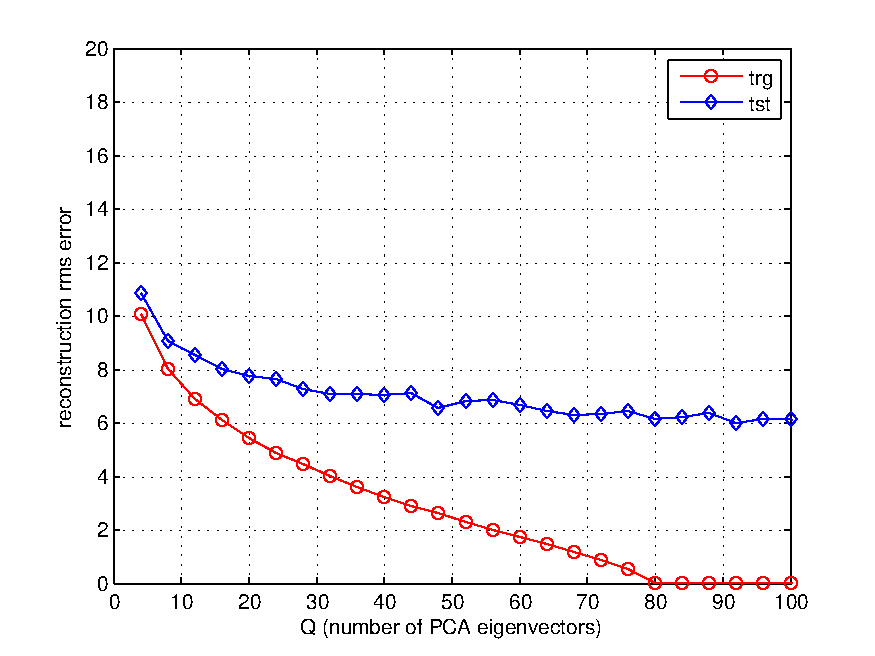
\includegraphics[width=0.45\textwidth]{figs/PCA_Dudek.pdf}}\hspace{0.2in}
\subfigure[Uniform random variable $U\sim$ \texttt{[}0, 1\texttt{]} in $\mathbb{R}^{1089}$, 100 realizations.]{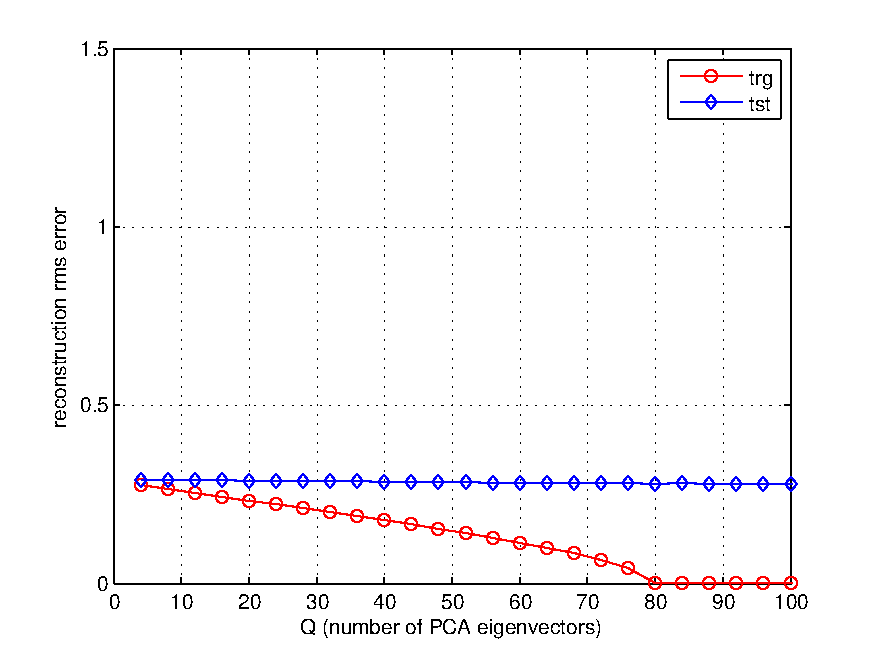
\includegraphics[width=0.45\textwidth]{figs/PCA_Uniform.pdf}}
\subfigure[Gaussian random variable $\mathcal{N}\sim$(0, 1) in $\mathbb{R}^{1089}$, 100 realizations.]{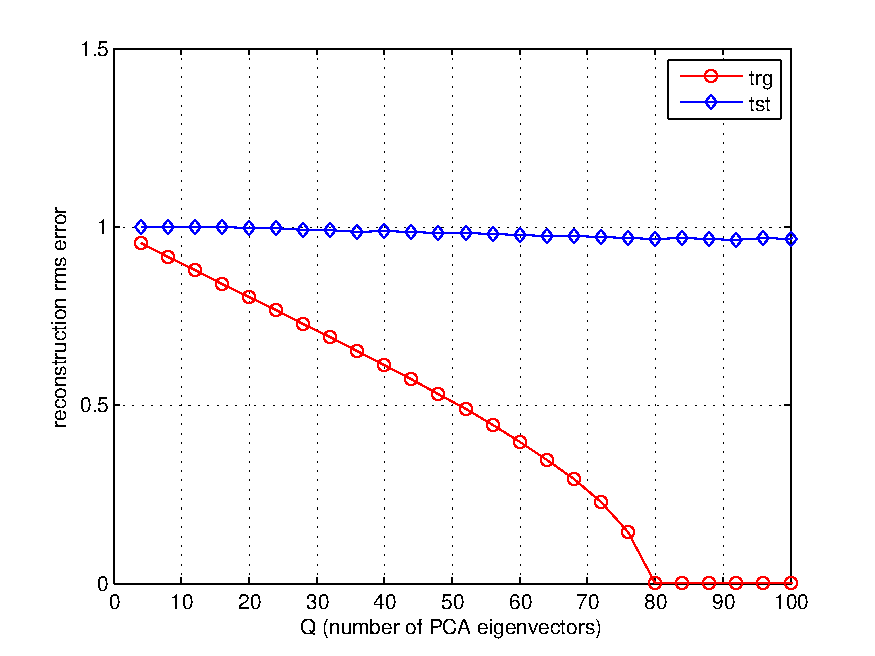
\includegraphics[width=0.45\textwidth]{figs/PCA_Gaussian.pdf}}\hspace{0.55in}
\subfigure[Gauss-Markov random variable $\mathcal{N}\sim$(0, 1) in $\mathbb{R}^{1089}$ with 0.9 correlation, 100 realizations.]{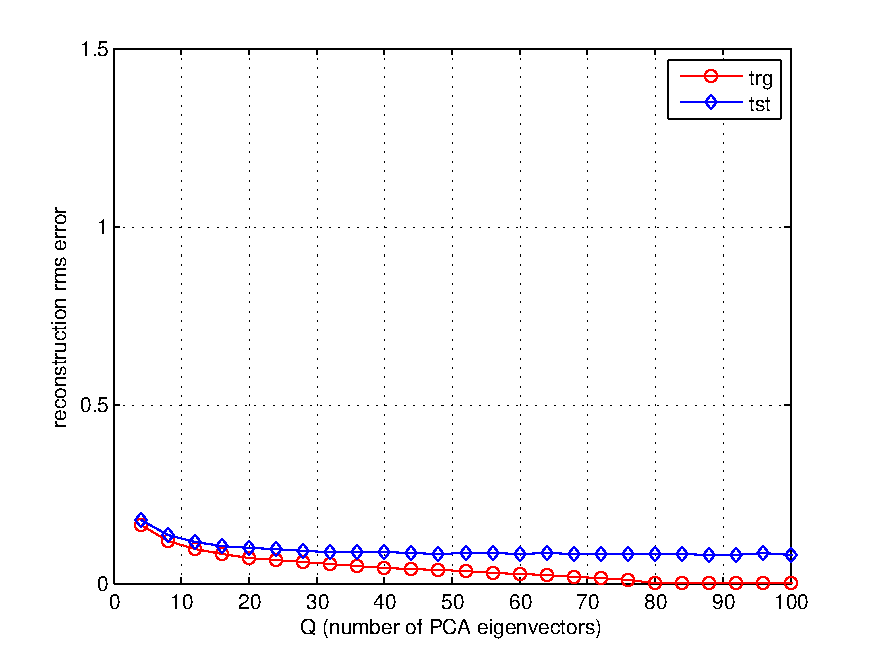
\includegraphics[width=0.45\textwidth]{figs/PCA_GaussMarkov.pdf}}
\caption{PCA experiments, 100 training examples in $\mathbb{R}^{1089}$ were used for each of these experiments.  Results were averaged over 10 cross-validation runs.  For each run, 20\% of the data, i.e., 20 examples were randomly picked for testing while the remaining 80 examples were used for training.}
\label{fig:PCA_results}
\end{figure}



\begin{figure}
\subfigure[Dudek sequence, 33x33 ($\mathbb{R}^{1089}$) face snippets were extracted from the first 100 images.  The ground truth affine parameters $\theta, \lambda_1, \lambda_2, t_x, t_y$ used to extract the snippets from the images were corrupted with zero-mean additive gaussian-noise (standard deviation 0.1) to simulate the effect of errors in tracking estimates.]{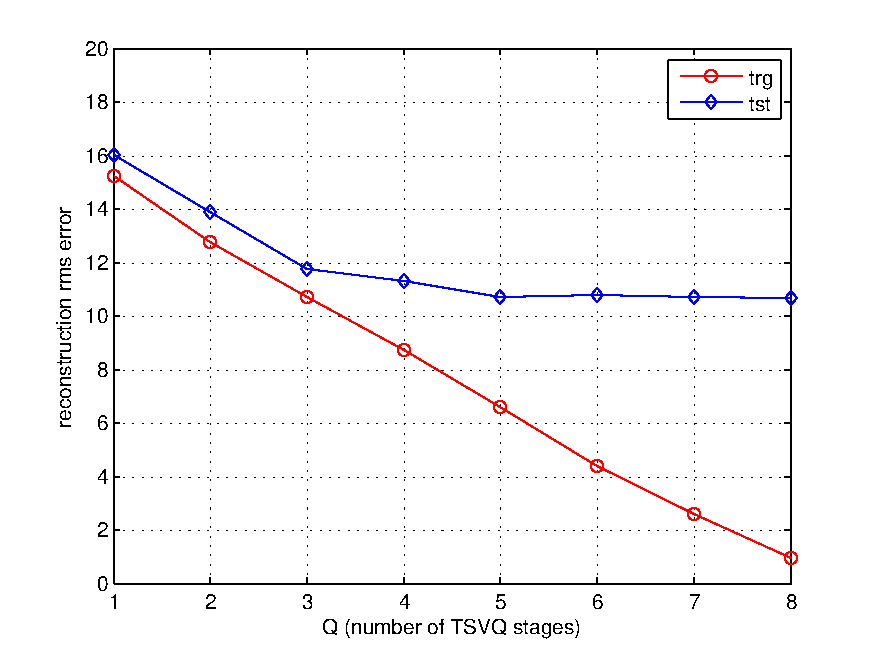
\includegraphics[width=0.45\textwidth]{figs/TSVQ_Dudek.pdf}}\hspace{0.2in}
\subfigure[Uniform random variable $U\sim$ \texttt{[}0, 1\texttt{]} in $\mathbb{R}^{1089}$, 100 realizations.]{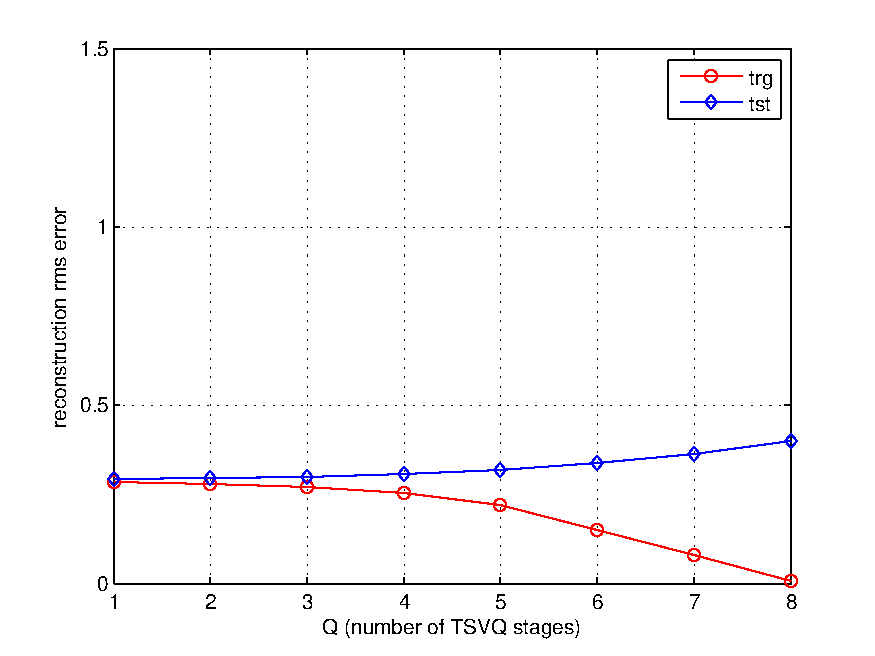
\includegraphics[width=0.45\textwidth]{figs/TSVQ_Uniform.pdf}}
\subfigure[Gaussian random variable $\mathcal{N}\sim$(0, 1) in $\mathbb{R}^{1089}$, 100 realizations.]{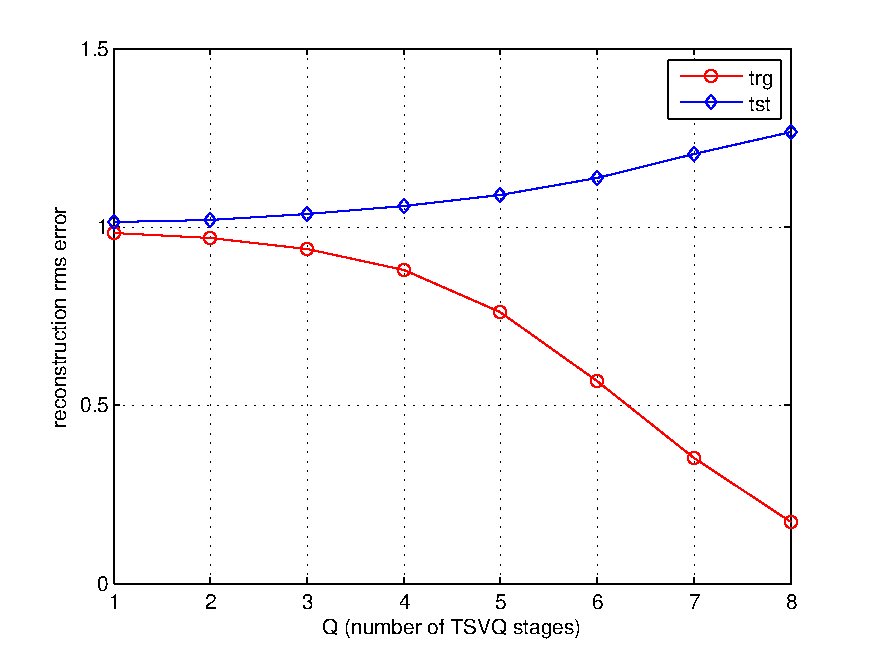
\includegraphics[width=0.45\textwidth]{figs/TSVQ_Gaussian.pdf}}\hspace{0.55in}
\subfigure[Gauss-Markov random variable $\mathcal{N}\sim$(0, 1) in $\mathbb{R}^{1089}$ with 0.9 correlation, 100 realizations.]{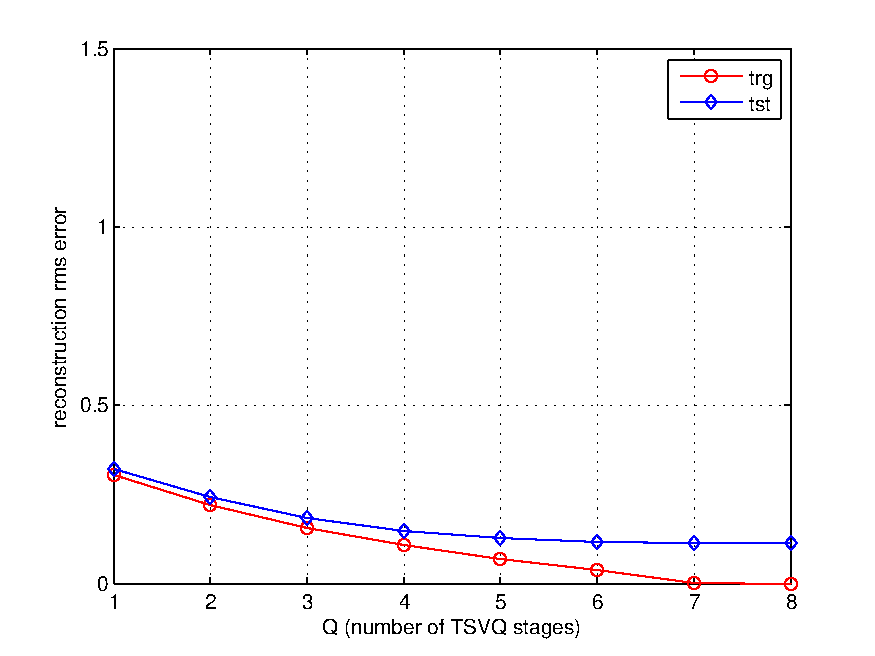
\includegraphics[width=0.45\textwidth]{figs/TSVQ_GaussMarkov.pdf}}
\caption{TSVQ experiments, 100 training examples in $\mathbb{R}^{1089}$ were used for each of these experiments.  Results were averaged over 10 cross-validation runs.  For each run, 20\% of the data, i.e., 20 examples were randomly picked for testing while the remaining 80 examples were used for training.}
\label{fig:TSVQ_results}
\end{figure}


%=========================
\section{Conclusions}
%=========================
\subsection{PCA}
In all 4 cases, the training error decreases monotonically with increasing eigenvectors.  This is expected, even in the random datasets since more and more eigenvectors continue to explain the data until the training error becomes 0 when 80 eigenvectors are used, since there are 80 training examples.  Also, for all cases, the test error decreases at a slower rate than test error as expected. 

For the Dudek sequence, we see that the test error decreases up till about 50 eigenvectors and then levels off.  This means that it takes about 50 eigenvectors to capture most of the linear dependencies in this dataset.  After the 50 eigenvector mark, the test error does not increase since the test vectors are very similar to the training set.  This is what one would expect in a tracking scenario over short periods of time.  

For the uniform, Gaussian, and uniform random variable cases, PCA test error stays about the same since there is no statistical correlation in the data.  For the Gaussian source, the error is equal to the variance of the source.  For the Gauss-Markov case, test error drops and then levels off.  This is expected since the Gauss-Markov has first order linear dependency.

\subsection{TSVQ}
For the binary balanced-tree TSVQ, test error and training error for the Dudek and Gauss-Markov cases decrease as expected with increasing stages.  However, for the datasets in which there is no correlation, TSVQ test error increases monotonically.  It appears that the TSVQ code-book is over-trained.  Since the test data is quite different from the training data, test error starts to increase.  

\subsection{Overall}
Overall, the test error for low Q in PCA and low Q in TSVQ is about the same.  However, TSVQ with its high VC dimension as the number of stages goes up starts to over-generalize.

\normalsize
\bibliographystyle{ieee}
\bibliography{MyCitations}
\end{document}